\documentclass{llncs} %
\bibliographystyle{splncs}
\usepackage{url}
\usepackage{graphicx}
\usepackage{lscape}

\newcommand{\source}[1]{\hfill Source: {#1} }

\begin{document}

\title{Supporting meditation training with EEG headsets}
\author{Vincenzo Pace}
\institute{Karlruhe Institute of Technology, Karlsruhe, Germany}
\maketitle
\newpage
\section{Abstract}
Adoption and functionality of wearable devices are increasing and expected to continue to do so \cite{Patel}. In the west, meditation is accepted more widely as a means of health improvement \cite{Tang:et al}.
Consumer EEG devices and freely available EEG/ERP databases \cite{ucsd} offer a chance to use algorithms to analyze a user's meditation experience and provide feedback for improvement.
This work seeks out to answer the question whether consumer grade EEG devices are feasible to be used as a tool in everyday meditation practice and through what mechanisms they could provide a benefit to the user. Thus, the underlying neuroscience and signal measurement and processing will be roughly presented. Ideally, an App could be made to facilitate all the results of scientific research to provide the function of a meditation "coach". 
\medskip

In the end, three popular EEG headsets will be compared and evaluated.
\section{Introduction}
\subsection{EEG}
EEG stands for electroencephalography and is a process to record the electrical activity in the brain. The measured signal are voltage changes in and between neurons. EEG can only measure signal in the outer regions of the brain \cite{Sitaram}.
The brains signal is in the order of mikrovolt \cite{Berger}. For measurement, EEG electrodes are placed on the test subjects scalp. In Research, up to 256 electrodes are used \cite{Seeck}, while consumer grade devices use around 10\% of that \cite{Maskeliunas}.
The electrical signal is measured as frequencies and goes through an EEG ampflifier. These get passed to a Fast Fourier Transformation (FTT) or wavelet transformation \cite{Akin} to produce distinct waves, which are then categorized according to known patterns \cite{Shaker}.
Brain waves of individuals can be compared to aggravated data of many test subjects, to search for disorders \cite{Loo} or match for meditation success \cite{Tang:et al}, access to enough datapoints assumed.
There are four main brain frequencies \cite{Cahn}:
% quantitative eeg 
\begin{itemize}
    \item 
    Beta Waves (frequency range from 14 Hz to about 30 Hz), associated with intellectual activity and outwardly focused concentration
    \item 
    Alpha Waves (frequency range from 7 Hz to 13 Hz), associated with relaxation
    \item 
    Theta Waves (frequency range from 4 Hz to 7 Hz), associated with mental inefficiency \cite{Hammond}, zone between wake and sleep
    \item 
    Delta Waves (frequency range up to 4 Hz), associated with sleeping, learning disabilities \cite{Hammond}
\end{itemize}
From the data, conclusions about attention \cite{Berka}, stress \cite{Hosseini}, cognitive load \cite{Antonenko} and more are possible, but infering the state of relaxation from sole EEG signals is difficult if not controversal \cite{Maskeliunas}. Quantitative EEG is the field that deals with these kind of calculations.
While EEG caps are usually used in research and academia \cite{Seeck}, headsets provide a reasonable solution for consumers with less complexity, but also lower precision\cite{Maskeliunas}.
For the accuracy of the measurement it is crucial, that the sensors are correctly affixed \cite{Seeck}, to accurately measure the brain regions that are involved in meditation.
\medskip

EEG devices are either gel based or dry. In Research, gel electrodes are used and cost thousands of dollars, have wired signal transmission and are time consuming to set up and are uncomfortable to wear.
Consumer devices on the other hand are dry, wireless and cost only a few hundreds of dollars. \cite{Decho}
\subsection{Neurofeedback}
Neurofeedback (NFB), also called EEG biofeedback, is a therapy that was invented as a method for training brainwave patterns through operant conditioning and is known since the 1960s \cite{Hammond}. 
It is used not only as a treatment of disorders \cite{brand:del}, but also in peak performance training \cite{Kaufman}. NFB experiments led to the deleopment of the field of brain-machine interfaces \cite{Sitaram}. 
Operant conditioning is the learning process where a behavior is modified by punishment or reward \cite{Spence}. NFB never uses punishment though. In NFB, the neural activity is recorded and presented to the participant in real time, either auditory or visual.  
Usually people are not aware of their brain waves, so seeing them on a screen helps by giving you the ability to see the results of your behavior and thus working towards control of them. This is the operant conditioning part. In the beginning, the changes are only short-lived, but with practice can become lasting. 

\begin{figure}
    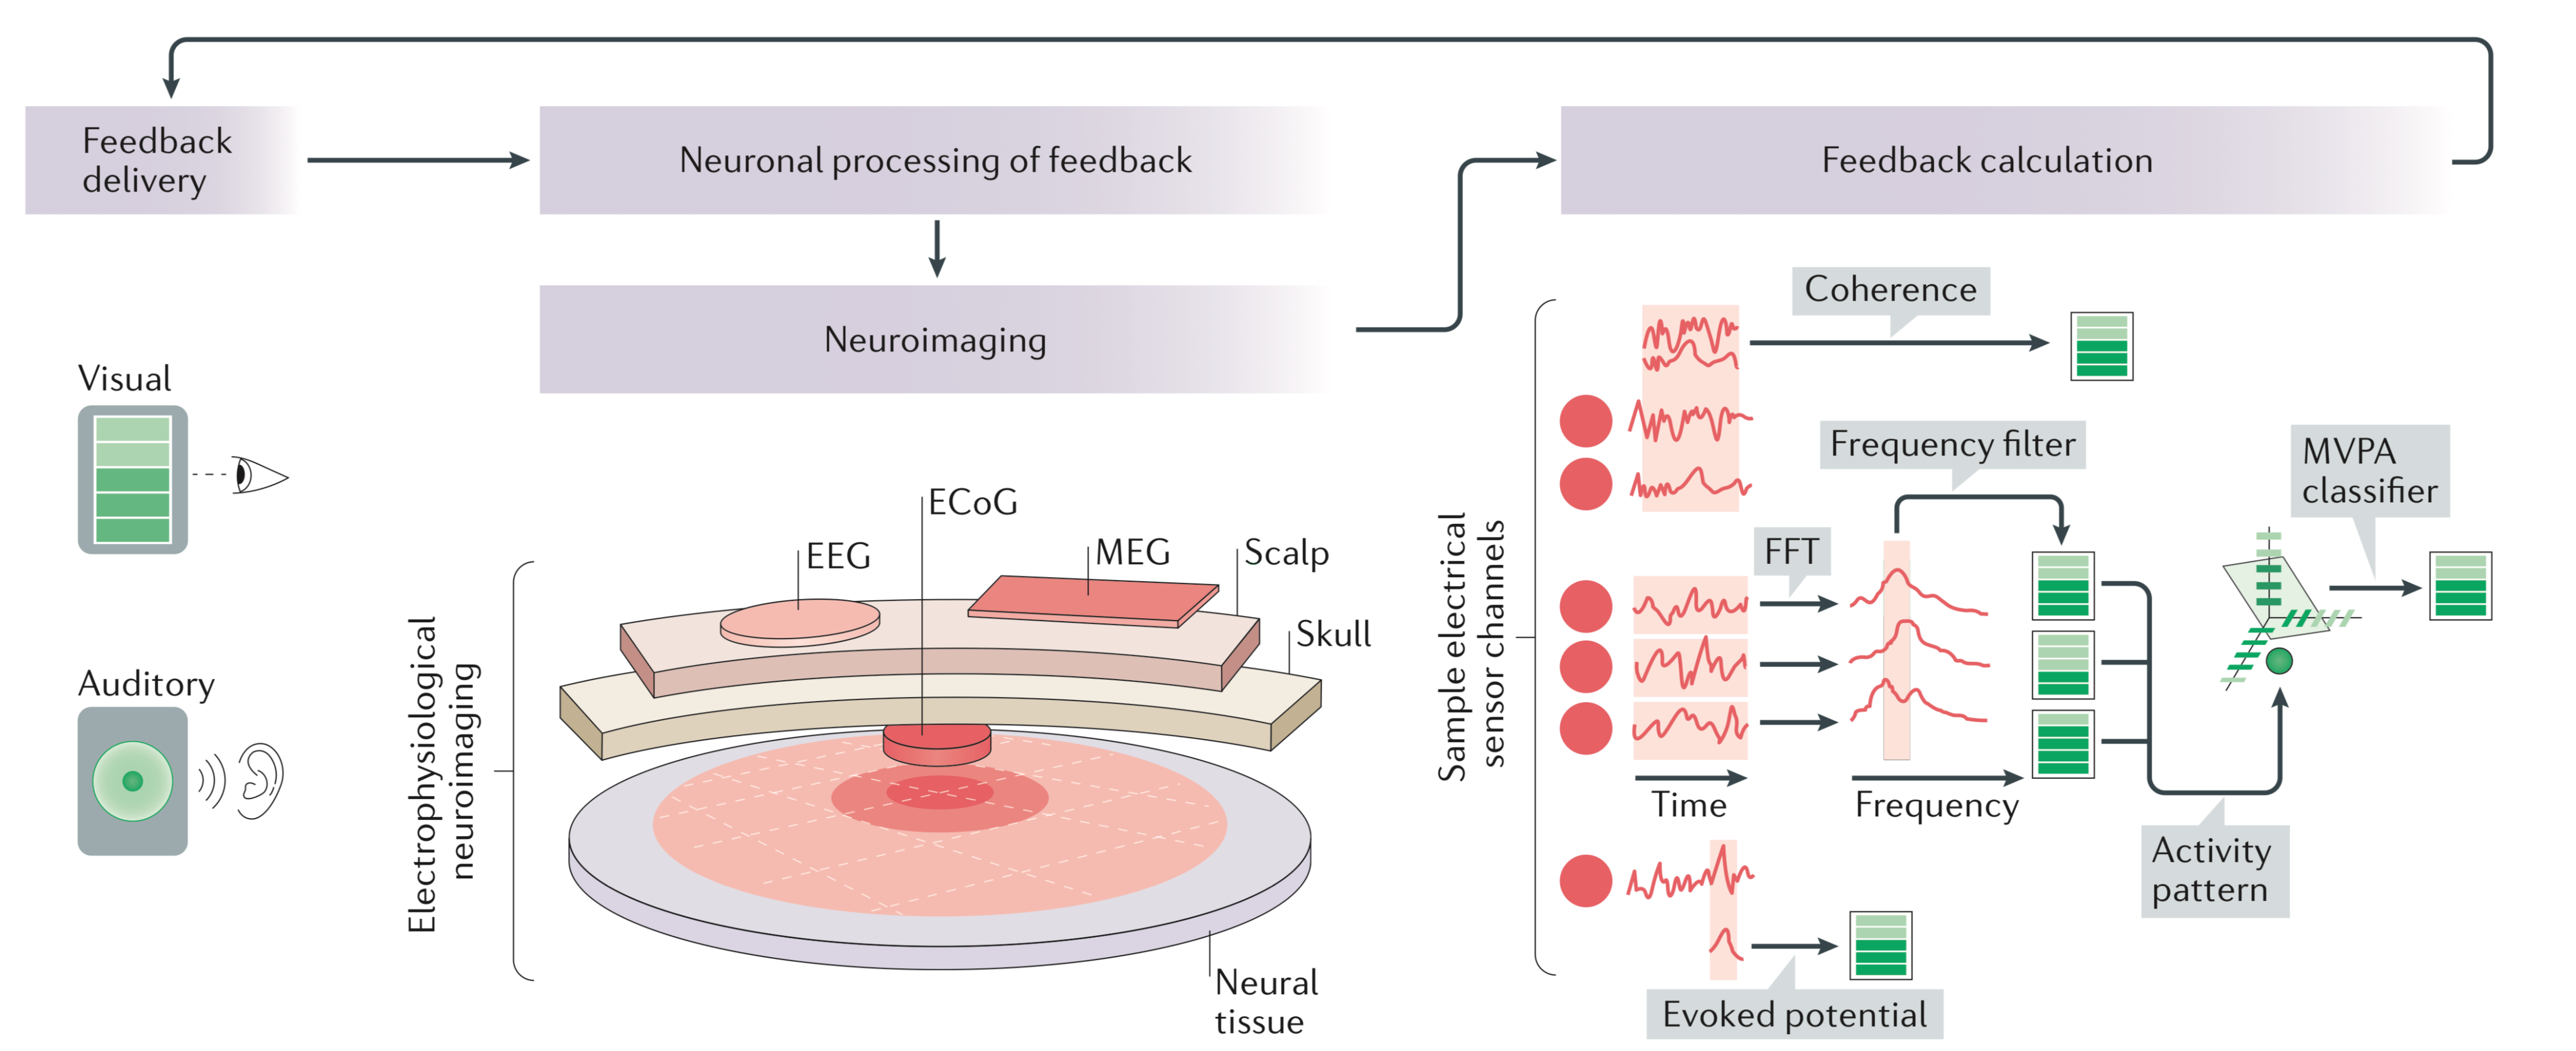
\includegraphics[width=\linewidth]{Neurofeedback.png}
    \caption{The neurofeedback process}  
    \label{neurofeedback}
    \source{Sitaram et al, 2016}
\end{figure}

NFB is non-invasive and is sometimes used as an alternative to medication \cite{Hammond}. Another unique kind of NFB is called LENS (Low Energy Neurofeedback System), where a tiny electromagnetic signal is introduced to the electrodes and transported to the brain.
However, it is not recommended to use NFB equipment without any expertise. Also, the training should be individualised to the unique brainwave patterns of each person. A physician should always be consulted first.
Otherwise, negative side effects or degradation of existing disorders are possible. Only healthy individuals should use a NFB device for meditation training on their own risk.

\subsection{Meditation}
Over the last decades, meditation has gained the interest of popular culture and the scientific community.
Documented beneficial effects range from mood improvements to structural changes \cite{Davidson} in various regions of the brain, such as the amygdala (responsible for stress and anxiety), anterior cingulate cortex, brain stem (breathing)
and the default mode network \cite{Tang:et al}.
Therefore, meditation has become part of psychiatric interventions \cite{Hoelzel}, high performance sports and personal development.
Historically, meditation stems from buddhist practices and has been part of eastern culture for centuries, while variations were also practiced by the ancient greeks \cite{Hadot:Davidson}.
\medskip

Although there is not one single meditation practice, the methods are plentiful. While often associated with stillness and watching ones breath,
there are also more active forms of meditation that involve more movement. Travis and Shear categorize meditation practices into focused attention, open monitoring and automatic self-transcending.\cite{Travis} 
Most of the papers analysed for this literary research deal with 'mindfulness meditation', which is a blend of focused attention and open monitoring meditation. In focused attention, there is usually an object like the breath, where practicioners put their attention on. Open monitoring meditation is about noticing how the body and mind feel.
\medskip

For the sake of this evaluation, the differences are not of greatest importance, but categorization of the different meditative practices is possible based on the measured EEG data. In a possible app scenario, this would definitely be a sought after feature to train specifically a certain meditation practice.
\subsection{Awareness}
Mindfulness and awareness are two terms often mentioned in the context of meditation and there is no single scientific definition to separate these two. Merriam Webster lists the two terms as synonimous and defines awareness as: "knowledge and understanding that something is happening or exists" \cite{Merriam:Webster}. 
\medskip

In current research contexts, mindfulness is typically defined as nonjudgmental attention to experiences in the present moment \cite{Kabat-Zinn}. In the studies that investigate mindfullness meditation, this awareness is self-reported by the participants. Usually, participants report when they notice that they have lost focus on their object of meditative focus. This feedback is then manually matched up with the measured signal.
\newpage
\section{Goals}
Since the beneficial effects of meditation are so various, the goals of using a wearable device 
that provides neurofeedback to its user are inherently diverse. Machine assisted meditation could help individuals to 
improve faster, track their progresssion, analyze the state of mind and lower the entrance barrier for novel practicioners. \cite{brand:del}
All of these different features can be combined in an app targeted at consumers. 
The differences in EEG signals induced by the different meditation practices enable a categorization
and dedicated training regime to offer the device and software solution to a wider audience. \cite{Travis}
\section{Measurement Data}
There is a wide array of different biological signals that change according to phyisical or mental activity, mental or emotional states and surroundings. Almost all of them can be measured very precisely in a research environment with high-end technical equipment, but not all of them have the same relevancy or are feasible to be involved in the consumer area. The most accurate results are given by measurements that examine brain activity, since the brain regions involved in meditation are well understood and categorized and can be specifically linked to observed data. Heart rate, skin conducatance and others on the other hand, are more general and can only be linked with confidence to broader mental states such as stress or relaxation. 
\medskip

Using too many signals will certainly lower the quality of any model that is trained on the given data. The goal is to identify the principal components that contribute the most information about the ongoing meditation state and the observable signals in the body and brain. 
\medskip

Below are all signals or measurement techniques listed that have been widely used in meditation research. 

\begin{landscape}
    \begin{table}[]
    \begin{tabular}{|l|l|l|}
    \hline
    Signal / Measuring Technique                                                                                                            & Relevancy                                                                                                                                                                                                                                                                                                                                                       & Feasability                                                                                                                                                                                                                                        \\ \hline
    EEG                                                                                                                                     & \begin{tabular}[c]{@{}l@{}}By far the most relevant signal. \\ Most studies rely solely on EEG signals.\end{tabular}                                                                                                                                                                                                                                            & \begin{tabular}[c]{@{}l@{}}There is a vast body of data available\\ to train machine learning\\ algorithms on EEG signals. \\ Research EEG devices measure the \\ signal very accurately,\\ while consumer grade devices are lacking.\end{tabular} \\ \hline
    \begin{tabular}[c]{@{}l@{}}Functional near-infrared \\ spectroscopy (fNIRS)\\ Measures oxygen in the blood\\ in the brain.\end{tabular} & \begin{tabular}[c]{@{}l@{}}Used in many meditation studies and\\ adds valuable information to gain further insight.\end{tabular}                                                                                                                                                                                                                                & \begin{tabular}[c]{@{}l@{}}As of now, there are no devices \\ available for consumers. \\ The setup is complicated, \\ but the data can be used to produce data.\end{tabular}                                                                      \\ \hline
    \begin{tabular}[c]{@{}l@{}}Electrocorticography (ECoG)\\ Measure electricity on the brain\\ with open skull\end{tabular}                & \begin{tabular}[c]{@{}l@{}}Gives very precise results, \\ but very invasive and not worth the effort.\end{tabular}                                                                                                                                                                                                                                              & Can not be used by consumers.                                                                                                                                                                                                                      \\ \hline
    \begin{tabular}[c]{@{}l@{}}Magnetoencephalography (MEG)\\ \\ \\ Measures magnetic field changes \\ in the brain\end{tabular}            & \begin{tabular}[c]{@{}l@{}}Widely used in Brain mapping. \\ Gives good results in some studies \\ and adds another dimension.\end{tabular}                                                                                                                                                                                                                      & \begin{tabular}[c]{@{}l@{}}Needs big and expensive equipment. \\ Not suitable for consumers.\end{tabular}                                                                                                                                          \\ \hline
    Skin Conductance                                                                                                                        & \begin{tabular}[c]{@{}l@{}}There are measurable changes to skin \\ conductance as a reaction to stress. \\ This could in theory be done in \\ combination with other methods to add \\ another dimension. \\ But I do not believe the value to be very high.\\ Only stress is measured basically,\\ the subject can be relaxed without meditation.\end{tabular} & \begin{tabular}[c]{@{}l@{}}Measuring skin conductance with a \\ wearable device is easy.\end{tabular}                                                                                                                                              \\ \hline
    Heart Rate                                                                                                                              & \begin{tabular}[c]{@{}l@{}}The heart rate changes according to our \\ mental and physical state. \\ Maybe there are some patterns in the \\ Heart Rate Variability\\ once meditation state is achieved, \\ so that these can be learned from an algorithm\\ and be  matched against during future practice.\end{tabular}                                        & \begin{tabular}[c]{@{}l@{}}Almost every modern health wearable has \\ a heart rate monitor \\ and accuracy is rather high in devices \\ like the Apple Watch 5.\end{tabular}                                                                       \\ \hline
    Breath Rate                                                                                                                             & \begin{tabular}[c]{@{}l@{}}As the heart rate, the breath rate also changes\\ according to physical\\ and mental state. If the goal is a certain\\ way of breathing, this can be monitored\\ and used as another dimension.\end{tabular}                                                                                                                         & \begin{tabular}[c]{@{}l@{}}Using a device that is hooked to mouth \\ or nose is most likely\\ distracting from meditation\\ and not beneficial to the actual practice.\end{tabular}                                                                \\ \hline
    \end{tabular}
    \end{table}
    \end{landscape}

After looking at all the different kind of biological signals that are involved in meditation, the ones that seem to be the most promising are EEG devices because of their high availability, low cost and great support. fNIR devices add another level of precision to the measurement, so an optimal device would use both signals and feed the data to an algorithm that utilizes the additional fNIR dimension. Such devices already exist and are very new, but they are only available in research grade and are very expensive. \cite{ws} 
\medskip

Whether this combination will be accessible for consumers in the future remains to be determined. 
\subsection{Medical challenges}
To get reliable results of any kind of brain wave analysis, an expert has to measure and evaluate the baseline brainwave pattern of any individual. This process is called a Quantitative EEG Assesment and usually takes about 1.5 hours, which is too long and unfeasible for a consumer. There are no known and reliable ways to do an automatic DIY assessment with an App or such things. This requirement makes it extremely difficult to harness the availability of wearable devices and advancements in EEQ headset technology. 
Resulting from the necessity of expert supervision, a lawsuit from consumers is very likely if a developer tries to sell a product that claims to automate this process reliably and safely.
\medskip

Furthermore, involuntary movement of the tongue, eyeballs, jaw and facial muscles produce noise in the milivolt range, while brain signals are on  the order of mikrovolt. These artifacts do not only occur in consumer grade EEG devices, but also in medical grade.
These artifacts need to be filtered out to produce a reliable signal for further analysis \cite{Bashivan: et al}, which will be extremely difficult, since the device would need to know about the precise kind and timing of any movement during measurement \cite{Hammond}.
\medskip

Another underlying problem is more of a psychological than technological nature: No matter which algorithm we use for classification, prediction etc. and what method we use for the neurofeedback training, they are all based on theories. When neurofeedback was invented as a therapy method, it was very questionable and doubted by many researchers and doctors. Nowadays, it is a recognized and widely used therapy method, but the underlying neuroscientific processes in the brain involved in learning are still poorly understood. Such fundamental theories as the Hebbian Theory ("Neurons that fire together, wire together; while neurons that fire out of sync, lose their link") are currently receiving further scrutiny, particularly the second part \cite{Brown}. This only underlines the fact that all kinds of 'assisted learning' that are based on algorithms will fall when the respective theories are disproven or altered.
\medskip

Artifical neural networks (ANN) try to emulate how the human brain functions and learns. There is a wide array of different kinds of ANNs, because there are many pathways, patterns and mechanism how the brain learns. These are themselves associated with different learning theories and neuropsychological models. To write an algorithm that assists the user in meditation training, the developer has to decide on a learning theory to base his model on. And of course, the quality of the algorithm is based on the accuracy of the theory.
\medskip

Neurofeedback training may not always result in behavioural modifications. Studies in monkeys showed that the response of neurons in the motor cortex to operantly learned rewards are initially associated with active limb movements, but, as the monkey continues to activate the reward-linked neurons, the movements drop out entirely \cite{Sitaram}. 
\medskip

Subjects just learn upregulating and downregulating EEG instead of actual meditation. Or even worse, the natural brain wave pattern of an individual is lastingly altered, without any knowledge of the possible side effects. 
\medskip

Despite its promise, neurofeedback faces several challenges, including the failure of some individuals to achieve self-regulation, inter-individual differences in learning capacity, uncertain long-term effects and unclear transfer benefits. Indeed, a substantial proportion — up to 30\% — of participants in neurofeedback and Brain-Computer-Interface (BCI) studies fail to self-regulate specific brain activity even after repeated training.
\subsection{Technical challenges}

So far, I have focused on EEG headsets and their application in neurofeedback meditation training. But the EEG signal alone might not be enough \cite{Travis}. While it gives high quality measurement of brain wave signals, the blood-oxygen-level-dependent (BOLD) signal detected in fMRIs or fNIRs add an additional information vector that provides in-depth information of activity in the brain. While this would be very easy to include from a software engineering perspective (since it would only be another feature for the ANN), there are no consumer grade devices that measure both signals at the same time. Even in the research area, there is currently only one manufacturer that produces such devices as of recently. \cite{Sulzer}
\medskip

The accuracy of machine learning models is dependent on the time frame of measurement that is chosen. The window length used to generate samples has a decisive impact on the achievable performance of the trained model. Bashivan et. al received their best results with a 120 second window, but state that this might be too long for some applications \cite{Bashivan: et al}. In their paper, they analysed mental states with the hope to detect wether a driver is drowsy or or someone is tired of work. For this I believe the two minute time window to be appropriate, but for a real-time analysis of an active meditation session, this is far too long. The usual practicioner recognizes his own mental state far before that and can adjust himself. In addition comes the problem that the mental states during meditation are far more complex than simply detecting states like tiredness or sadness.
\medskip

It was common for inexperienced users to wear the device too low on the forehead so the electrodes were placed over a sinus cavity rather than brain. This led to weaker than expected reading for frontal signals. Users with thick hair typically had problems getting a good contact with the temporal electrodes \cite{Bashivan: et al}. Additionally, many users report pain or feel uncomfortable or distracted after wearing the devices for extended periods. 
\medskip

What is much less clear is whether and how meditation practices produce increased alpha beyond that obtained from reducing general arousal, which may become apparent only when fine-grained topographic mapping is combined with other neuroimaging methods \cite{Cahn}.

\subsection{Other challenges}
During meditation, the practicioner has to focus solely on meditating. Most neurofeedback systems provide auditory or visual feedback that fully engage and demand the attention of the subject \cite{brand:del}. During these sessions, the subject is usually presented a screen that directly shows him the movements of his brain wave patterns. If the practicioner looks at, evaluates and tries to adjust to the presented data, he will not have any capacity to practice meaningful meditation with the necessary concentration. 
\medskip

Audio feedback, such as a gentle voice similiar to the one used in the Headspace App \cite{Headspace}, could provide precise information about measured mental states and thus lead the subject in the 'correct' direction. Further research is necessary, to fully understand the impact of audio guidance on meditation training.
\medskip

Optimally, the feedback would be given to the practicioner in an unobstrusive way, such as haptic feedback in combination with devices such as the Apple Watch. Different patterns of soft vibration can be used to give different feedback, as is already used in the Apple Maps app to signal either turning left or right with haptic feedback that varies in intensity, length and frequency. 

\subsection{Processing and evaluation}

In the beginning, a continuous EEG signal is measured and samples are generated according to a predefined time frame. Depending on the goal of the experiment, the circumstances and the context, the windows can vary between a few seconds to a few minutes. 
\medskip

In real-time analysis, the signal that is extracted from these methods is typically transformed into the frequency domain and decomposed into a specific frequency (for example, delta (0–4 Hz), theta (4–7 Hz), alpha (8–12 Hz), beta (12–30 Hz) and gamma ($\geq$ 30 Hz) bands) before feature extraction. Examples of feature extraction include coherence, power spectral density and their combinations for input to multivariate patterns, event-related potentials and slow cortical potentials. The signals can be processed either in sensor space (that is, individual electrodes) or source space (for example, beam formers or LORETA) that enables a more accurate estimate of the activity in cortical regions that then is transformed into the feedback signal \cite{Sitaram}.
\medskip

After measuring the signals with EEG and possibly fNIRS devices, the signal goes preprocessing and feature extraction steps that are common in all kinds of signal processing. For EEG signals, Fast Fourier Transormation, Wavelet Transformation, and Independent Component Analysis are used for preprocessing, denoising and feature extraction. While the aforementioned are some widespread examples, there are many more methods to analyse EEG signals.
\medskip

Multivariate pattern analyses (MVPAs) was used to decode whole brain states associated with sustained attention while participants performed a cognitive task. The level of difficulty of this task was automatically adjusted based on the decoded brain state to improve vigilance \cite{Sitaram}.
\medskip

This processed and cleaned data is then funneled to neural networks, random forests or other classifiers. So far, no single approach has emerged to be the best above all. The superiority of one algorithm over another varies on a case by case basis and is best determined experimentally on a given dataset. 
\medskip

As for the evaluation itself, different machine learning models like Random Forest, Decision Trees, Support Vector Machines and ANNs have been used so far. The evaluation task itself is inherently a form of pattern recognition and suffer from the blackbox behavior effect that the field is experiencing in general. In the studies evaluated for this paper, the respective authors mostly just tried out different approaches with the goal to find out which one has the best accuracy. 
Dixit and Rohan find their classification approach is able to distinguish between the baseline and meditation state on a second-by-second basis with a mean balanced success rate of 75.7\% \cite{Dixit}. In generel, this seems to be the level of quality that is currently possible with consumer devices and the available datasets. With growing data and accessibility, the results are expected to result by sheer mass.

\section{Training procedure}
Learning to control brain activity in humans is determined by contingent feedback and reward, and potentially by verbal instructions and mental strategies (for example, use of imagery) that are suggested by the experimenter to the participant \cite{Sitaram}. 
\medskip

In neurofeedback training, the measured EEG data is presented visually or auditory to the user. Since meditation is in most practices done with closed eyes, visual presentation would only be distracting. With the combination of meditation, wearable devices and the target audience of consumers who want to improve their skill, haptic feedback becomes also a viable form of information presentation. Users could receive a sound or vibration if they lose focus or sync with the desired brain wave pattern. A sequence of vibrations could represent a certain pattern and enforce adaption to these brain wave patterns.
\medskip

Assuming that reliable and reproducible EEG signatures are associated with specific meditation practices, we may expect that training subjects to reproduce these signatures would support and strengthen their meditation practice.
Clinical neurofeedback protocols are aiming towards comparing patients’ EEG with large EEG data sets from normal subjects in order to produce a neurofeedback algorithm which rewards subjects (patients) whose EEG becomes closer to that of the normal population \cite{brand:del}.
\newpage
\section{Available Devices}
In the following sections, three consumer EEG headsets will be compared. The studies used as a basis of my analysis are a few years old. In a such a fast moving field, the information might already be outdated. While one device was best a few years ago, it might not even be sold today. Thus, I try to present more general features of devices in a certain price category. While I focus on consumer grade EEG headsets, I will also look into one research grade device. What is professional performance now, will likely be achievable in consumer electronics in a few years. Thus, this can be seen as an outlook of what might be used by software engineers soon.
\subsection{Neurosky - Mindwave Mobile 2}
This device costs around 100\$, has only one electrode, uses one reference at the ear and uses the same board at is predecessor, the TGAM1 module from 2010. No reliable research has been conducted with this 2018 device yet, but it gets advertised as the most cost effective solution for EEG-oriented research. The differences to the last version are only of small nature, so I will look at older published studies that used the first Mindwave device. The signal in the second version is processed 512 times per second, while the last version did 128 times per second \cite{Maskeliunas}\cite{Mindwave1}\cite{Mindwave2}. 
\medskip

To me, they seem to be more focused on the entertainment and gaming sector, instead of actual research.  The papers that used the predecessor did not atttest it high quality measurements or prediction abilities. 
\subsection{InteraXon Inc. - Muse 2}
On their website, the Muse 2 is immediately advertised as a product to be used for meditation and promised to 'teach the art of focus' \cite{Muse}. In comparison to the other devices, they clearly focus more on meditation practicioners. They use realtime audio feedback in combination with bluetooth headphones and their own app to guide their users. They classify mental states into the categories 'Active', Neutral' and 'Calm' and adjust their feedback to inform the user over the measured mental state, i. e. when the user achives 'a deep, restful focus on [his] breath for an extended period of time, [he]'ll start to hear birds singing'. Additionally, they use a gamification approach and award points for each meditation session and track the number of 'birds singing'. 
\medskip

Hardware-wise, they use 7 sensors. 2 on the forehead, 2 behind the ears and 3 reference sensors and measure EEG, heart rate (PPG + pulse oximetry), Movement (accelerometer) and Breath (PPG + gyroscope), so they include the most feature vectors into their analysis. 
\medskip

Their technology is used by NASA, MIT and others for brain research studies. The afforementioned paper by Bashivan et al. \cite{Bashivan: et al} used a Muse device during their experiment. The papers they showcase on their website do mostly use the device for measurement, not for active training. One paper uses it in active meditation training, but does not have a control group that undergoes regular, unassisted meditation training. This would be a very interesting study to conduct and I am excited for the results. 
\medskip

With a price of 269\$ and a money-back guarantee, they seem to be the ones with the most value and complete package for consumers, at least for the purposes discussed in this paper. 
\subsection{Emotiv - Insight 5}
EMOTIV is an award-winning San Francisco based BCI company founded in 2011. They target researchers, companies and consumers with their products. Several independent papers using their products have been published. They offer an App and multiple EEG headsets. The EMOTIV Insight 5 EEG headset is their consumer device with a price of 300\$. With their software, they provide detection of facial expressions, which are important in noise detection, and mental metrics such as stress and focus. The EEG sensor uses five channels, two references above the ears and is made of a semi-dry polymer that needs to be moistened before usage. The nine axis motion sensors detect head movements. \cite{Emotiv1}


\subsection{Emotiv - EPOC+}
The EPOC internally samples at a frequency of 2048 Hz, which then gets down-sampled to 128 Hz sampling frequency per channel, and sends the data to a computer via Bluetooth. It utilizes a proprietary USB dongle to communicate using the 2.4 GHz band. Prior to use, all felt pads on top of the sensors have to be moistened with a saline solution \cite{Kushaba}
The Emotiv EPOC is a high resolution, neuro-signal acquisition and processing wireless headset that monitors 14 channels of EEG data and has a gyroscope measure for 2 dimensional control. It seems to be the absolute top of the market and features a rich documentation for developers, a fully fledged API that is constantly under development and the company is established in the market. Many studies aside from meditation also use Emotiv hardware.
\medskip

With its size, it is less convenient to wear than the consumer EEG headsets.
\section{The optimal device}
The optimal device would be convenient to wear like a normal headset, it would work in combination with pre existing wearables like smart watches or fitness trackers, it would measure EEG and fMRI signal, it would have an accessible API hat makes it easy for app developers to produce a meditation app as is envisioned in this literature research and it would cost around 100\$ to be attractive and affordable for a wide populace. Such a device does not yet exist unfortunately. A device that is suitable for the described neurofeedback meditation training is useful for many applications, such as gaming and therapy. Most of today's devices also to try to aim for broader application, but their lack of precision makes their advertised usage in meditation training questionable. 
\medskip

However, Bashivan et al. believe that with the development of novel approaches, such as thin tattoo-type electrodes, EEG recording will become practical in a much wider spectrum of real-life scenarios, and that recognizing mental states using wearables devices will become much more widespread \cite{Bashivan: et al}. 
\section{Conclusion}
Improving meditation experience with neurofeedback and wearable technology is a multidisciplinary field that encompasses signal processing, neuroscience, data science and psychology. Neurofeedback as a means of therapy for disorders has been well established over the last decades. While positive results have been shown and critics of the practice are getting less and less, all experiments or therapies have been conducted under the guidance or supervision of experts. Self-therapy with neurofeedback is not recommended but strictly discouraged by neuroscientists. With consumer EEG devices the technology is developing in a direction where analysis of brain waves at home become possible and meditation practicioners might be tempted to "optimize" themselves in this regard, as has become the trend in many areas recently. Since the underlying principle of neurofeedback training is a targeted change of brain waves, the consequences of self-directed training are unforseeable and thus outweigh any potential benefit in my opinion. The algorithms used to analyse meditation states seem very generic and not well thought-out. They act like a blackbox and are manually corrected and rated by experts who observed meditations in practicioners themselves. This can not be done by consumers at home. 
\medskip

In my opinion, neither the technology, nor the science are ready for this endevour at this point. The future looks promising from a technological perspective, but the medical risks should discourage any developer of building such an app without thorough understanding of the brain, learning and neurofeedback.
\newpage
\begin{thebibliography}{[MT1]}
    \bibitem{brand:del}
    Tracy Brandmeyer, Arnaud Delorme,
    Meditation and neurofeedback
    Frontiers in Psychology, Article 688 (October 2013).
    \bibitem{Tang:et al}
    Tang, Yi-Yuan, Britta K. Hölzel, and Michael I. Posner. "The neuroscience of mindfulness meditation." Nature Reviews Neuroscience 16.4 (2015): 213-225.
    \bibitem{Bashivan: et al}
    Bashivan, Pouya, Irina Rish, and Steve Heisig. "Mental state recognition via wearable EEG." arXiv preprint arXiv:1602.00985 (2016).    
    \bibitem{Travis} 
    Travis, Fred, and Jonathan Shear. "Focused attention, open monitoring and automatic self-transcending: categories to organize meditations from Vedic, Buddhist and Chinese traditions." Consciousness and cognition 19.4 (2010): 1110-1118.
    \bibitem{Hoelzel}
    Hölzel, Britta K., et al. "How does mindfulness meditation work? Proposing mechanisms of action from a conceptual and neural perspective." Perspectives on psychological science 6.6 (2011): 537-559.
    \bibitem{Cahn}
    Cahn, B. Rael, and John Polich. "Meditation states and traits: EEG, ERP, and neuroimaging studies." Psychological bulletin 132.2 (2006): 180.
    \bibitem{Berger}
    Berger, Hans. "Über das elektrenkephalogramm des menschen." European archives of psychiatry and clinical neuroscience 87.1 (1929): 527-570.
    \bibitem{Seeck}
    Seeck, Margitta, et al. "The standardized EEG electrode array of the IFCN." Clinical Neurophysiology 128.10 (2017): 2070-2077.
    \bibitem{Maskeliunas}
    Maskeliunas, Rytis, et al. "Consumer-grade EEG devices: are they usable for control tasks?." PeerJ 4 (2016): e1746.
    \bibitem{Akin}
    Akin, Mehmet. "Comparison of wavelet transform and FFT methods in the analysis of EEG signals." Journal of medical systems 26.3 (2002): 241-247.
    \bibitem{Shaker}
    Shaker, Maan M. "EEG waves classifier using wavelet transform and Fourier transform." brain 2 (2006): 3.
    \bibitem{Antonenko}
    Antonenko, Pavlo, et al. "Using electroencephalography to measure cognitive load." Educational Psychology Review 22.4 (2010): 425-438.
    \bibitem{Berka}
    Berka, Chris, et al. "Real-time analysis of EEG indexes of alertness, cognition, and memory acquired with a wireless EEG headset." International Journal of Human-Computer Interaction 17.2 (2004): 151-170.
    \bibitem{Hosseini}
    Hosseini, Seyyed Abed, and Mohammad Ali Khalilzadeh. "Emotional stress recognition system using EEG and psychophysiological signals: Using new labelling process of EEG signals in emotional stress state." 2010 international conference on biomedical engineering and computer science. IEEE, 2010.
    \bibitem{Loo}
    Loo SK, Barkley RA. Clinical utility of EEG in attention deficit hyperactivity disorder. Appl Neuropsychol 2005; 12(2): 64-76.
    \bibitem{Davidson}
    Davidson, Richard J., and Antoine Lutz. "Buddha's brain: Neuroplasticity and meditation [in the spotlight]." IEEE signal processing magazine 25.1 (2008): 176-174.
    \bibitem{Decho}
    Surangsrirat, Decho, and Apichart Intarapanich. "Analysis of the meditation brainwave from consumer EEG device." SoutheastCon 2015. IEEE, 2015.
    \bibitem{Hadot:Davidson}
    Hadot, Pierre; Arnold I. Davidson (1995) Philosophy as a Way of Life: Spiritual Exercises from Socrates to Foucault ISBN 0-631-18033-8 pages 83-84
    \bibitem{Patel}
    Patel, Mitesh S., David A. Asch, and Kevin G. Volpp. "Wearable devices as facilitators, not drivers, of health behavior change." Jama 313.5 (2015): 459-460.
    \bibitem{ucsd}
    \url{https://sccn.ucsd.edu/~arno/fam2data/publicly_available_EEG_data.html}, accessed on Nov 27, 2019
    \bibitem{Hammond}
    Hammond, D. Corydon. "What is neurofeedback?." Journal of neurotherapy 10.4 (2007): 25-36.
    \bibitem{Sulzer}
    Sulzer, James, et al. "Real-time fMRI neurofeedback: progress and challenges." Neuroimage 76 (2013): 386-399.
    \bibitem{Spence}
    Spence, Kenneth Wartenbee. Behavior theory and conditioning. Vol. 35. New Haven: yale university Press, 1956.
    \bibitem{Sitaram}
    Sitaram, Ranganatha, et al. "Closed-loop brain training: the science of neurofeedback." Nature Reviews Neuroscience 18.2 (2017): 86.
    \bibitem{Dixit}
    Dixit, Rohan. "Meditation training and neurofeedback using a personal EEG device." 2012 AAAI Spring Symposium Series. 2012.
    \bibitem{Merriam:Webster}
    \url{https://www.merriam-webster.com/dictionary/awareness}, accessed on Nov 29, 2019
    \bibitem{Kabat-Zinn}
    Kabat-Zinn, Jon, and Thich Nhat Hanh. Full catastrophe living: Using the wisdom of your body and mind to face stress, pain, and illness. Delta, 2009.
    \bibitem{Kaufman}
    Kaufman, Keith A., Carol R. Glass, and Diane B. Arnkoff. "Evaluation of Mindful Sport Performance Enhancement (MSPE): A new approach to promote flow in athletes." Journal of Clinical Sport Psychology 3.4 (2009): 334-356.
    \bibitem{Emotiv1}
    \url{https://www.emotiv.com/insight/}, accessed on Nov 29, 2019
    \bibitem{Mindwave1}
    \url{https://store.neurosky.com/pages/mindwave}, accessed on Nov 29, 2019
    \bibitem{Mindwave2}
    \url{http://wearcam.org/ece516/neurosky_eeg_brainwave_chip_and_board_tgam1.pdf}, accessed on Nov 29, 2019
    \bibitem{ws}
    \url{https://wearablesensing.com/products/dsi-hybrid-eegfnir/}, accessed Jan 19, 2020
    \bibitem{Brown}
    Brown, Richard E., and Peter M. Milner. "The legacy of Donald O. Hebb: more than the Hebb synapse." Nature Reviews Neuroscience 4.12 (2003): 1013-1019.
    \bibitem{Headspace}
    \url{https://www.headspace.com/}, accessed on Feb 5, 2020
    \bibitem{Muse}
    \url{https://choosemuse.com/muse-2/}, accessed on Feb 5, 2020
\end{thebibliography}
\end{document}